\documentclass{article} % For LaTeX2e
\usepackage{../../tex-style/nips_2014,times}
\usepackage{hyperref}
\usepackage{url}
\usepackage{graphicx}
\usepackage{CJKutf8}
\hypersetup{unicode}
\AtBeginShipoutFirst{\input{zhwinfonts.tex}}
\usepackage{algorithm}  
\usepackage{algorithmic}
\usepackage{amsmath}
\title{Playing Atari with Deep Reinforcement Learning}

\author{
 \url{http://www.dosrc.com/}
}


\nipsfinalcopy % Uncomment for camera-ready version

\begin{document}
\begin{CJK*}{UTF8}{gkai}

\maketitle

\section{相关知识}
马尔可夫决策过程

Atari 2600:雅达利(Atari)在1977年10月发行的一款游戏机,在当年风行一时,成为电子游戏第二世代的代表主机。当中经典的游戏包括Adventure、碰碰弹子台、爆破彗星和Pac-Man等。早期采用1.19MHz MOS 8位元6507处理器,后期升级到2MHz 6502处理器。支持160 X 192分辨率屏幕,最高128色,当然,还有主机上有128 bytes的RAM和6Kb的ROM内存。游戏盘每个售价25美元,容量4KB,不过通过技术手段可以使卡带达到10K的容量。

\section{简介}
直接从传感器传来的裸数据中学习控制智能体的策略一直以来都是强化学习的一个巨大挑战。
深度学习的突破性进展使得从裸数据中提取特征成为可能,这为计算机视觉,语音识别带来重大突破,它们(计算机视觉,语音识别)使用了一系列神经网络的架构,包括卷积神经网络,多层感知机,限制玻尔兹曼机,循环神经网络,既有使用监督学习,也有使用非监督学习。那么我们自然会问这一技术是否能为强化学习带来些什么。

然而从深度学习的视角来看,强化学习结合深度学习面临着一些困难:

\paragraph{1.}大部分成功的深度学习应用可能需要大量手工标注数据一样(这些深度学习算法从训练数据的标签中学习),同样强化学习的奖励信号也有着稀疏,噪声,延迟的问题(这些强化学习算法从奖励信号中学习),有时候奖励信号可能会延迟上千个迭代步之后才到来,这就使得学习输入和目标输出之间的联系变得异常困难。

\paragraph{2.}大部分的深度学习算法假设数据样本之间是独立的,且分布是固定不变的,然而强化学习中的数据大都是相关的,而且数据的分布会随着学习的进行而改变。

本文证明了卷积神经网络可以克服这些困难,从视频裸数据中学习到控制策略。该神经网络使用Q学习算法的一个变种进行训练,使用梯度下降算法更新权重。为了缓和数据相关和分布不固定的问题,我们使用了经验回放机制(experience replay mechanism),即通过多次随机采样之前的状态转移,来平滑训练分布的变化。

\section{Deep Reinforcement Learning}
许多强化学习算法的基本思想是估计动作值函数(Q函数),利用Bellman等式的值迭代算法可以收敛于最优的动作值函数。但是在实际中很难应用,所以我们经常使用函数逼近来估计值函数。在强化学习领域我们经常使用线性函数来做近似,但是非线性函数比如神经网络,有时也会使用,本文中我们使用一个带权重参数$\theta$的神经网络,称之为Q网络,我们通过最小化一系列的损失函数$L _{i} \left(\theta _{i}\right)$值来训练网络,我们定义损失函数如下:
$$L _{i} \left(\theta _{i}\right)=E _{s,a\sim \rho \left(\cdot\right)}\left[\left(y _{i} - Q\left(s,a;\theta _{i}\right)\right) ^{2}\right]$$
其中$y _{i}=E _{s ^{\prime} \sim S}\left[r+\gamma \max _{a ^{\prime}}Q \left(s ^{\prime},a ^{\prime};\theta _{i-1}\right)\vert s,a\right]$是第$i$次迭代的目标输出,$\rho\left(s,a\right)$是状态$s$下动作$a$的概率分布,称之为动作分布。

对损失函数求梯度得:
$$\nabla _{\theta _{i}}L _{i} \left(\theta _{i}\right)=E _{s,a\sim \rho \left(\cdot\right);s ^{\prime} \sim S}\left[\left(r+\gamma \max _{a ^{\prime}}Q \left(s ^{\prime},a ^{\prime};\theta _{i-1}\right) - Q \left(s,a;\theta _{i}\right) \right)\nabla _{\theta _{i}}Q \left(s,a;\theta _{i}\right)\right]$$

由于观察只观察当前画面几乎不可能完全理解当前所处的环境,所以我们定义状态为$$s _{t} = x _{1},a _{1},x _{2},\dots,a _{t-1},x _{t}$$
\subsection{Algorithm}
\begin{algorithm}
    \caption{Deep Q-learning with Experience Replay}
    \label{alg1}
    \begin{algorithmic}
        \STATE Initialize replay memory $D$ to capacity $N$
        \STATE Initialize action-value function $Q$ with random weights
        \FOR{$episode = 1,M$}
            \STATE Initialise sequence $s_{1}=\left\lbrace x _{1} \right\rbrace$ and preprocessed sequenced $\phi _{1}=\phi\left(s _{1}\right)$
            \FOR{$t=1,T$}
                \STATE With probability $\epsilon$ select a random action $a _{t}$
                \STATE otherwise select $a _{t}=\max _{a}Q ^{*}\left(\phi\left(s _{t}\right),a;\theta\right)$ 
                \STATE Execute action $a _{t}$ in emulator and observe reward $r _{t}$ and image $x _{t+1}$
                \STATE Set $s _{t+1}=s _{t},a _{t},x _{t+1}$ and preprocess $\phi _{t+1}=\phi\left(s _{t+1}\right)$
                \STATE Store transition $\left(\phi _{t},a _{t},r _{t},\phi _{t+1}\right)$ in $D$
                \STATE Sample random minibatch of transitions $\left(\phi _{j},a _{j},r _{j},\phi _{j+1}\right)$ from $D$
                \STATE Set $y _{j}=
                    \begin{cases}
                        r _{j}& \text{for terminal $\phi _{j+1}$}\\
                        r _{j} + \gamma \max _{a ^{\prime}}Q\left(\phi _{j+1},a ^{\prime};\theta\right)& \text{for non-terminal $\phi _{j+1}$}\\
                    \end{cases}$
                \STATE Perfoem a gradient descent step on $\left(y _{i}-Q\left(\phi _{j},a _{j};\theta\right)\right) ^{2}$ according to $\nabla _{\theta _{i}}L _{i} \left(\theta _{i}\right)$
            \ENDFOR
        \ENDFOR
    \end{algorithmic}
\end{algorithm}
\subsubsection{优点}
\paragraph{1.}每一次与环境交互的经验被多次的用于更新权重,数据使用率高
\paragraph{2.}打散了数据,使得数据之间的关联性降低
\paragraph{3.}由于当前的参数会影响下一次与环境的交互数据,例如最优的策略是向左边动,那么接下来的一系列训练数据会被向左给主导,经验回放机制可以避免陷入局部最优,减小训练参数的动荡和分散度。
\subsubsection{缺点}
\paragraph{}由于记忆储存容量有限,我们只存储最后的N次经验,采用的是先进先出队列的模式存储,没有区分哪次状态转换比较重要。
\subsection{预处理和模型框架}
\textbf{预处理:} Atari游戏的每一帧都是128色210*160像素的图像,直接处理这么大的数据会对计算能力要求比较高,为了减小输入数据的维度,我们对数据进行了预处理,将RGB色彩转换为灰度级并下采样。alogrithm 1中的$\phi$函数就是进行这种预处理的函数,它只处理了状态$s$历史信息的最后四帧,处理的结果作为输入。

\textbf{模型框架:}
由于$Q\left(s,a\right)$包含$s$和$a$。之前的一些方法是输入$s$和$a$到深度神经网络,输出$q$值,但是这样的话每个a都需要forward一遍网络。
我们的做法是神经网络只输入s,输出则是每个a对应的q。这种做法的优点就是只要输入s,forward前向传播一遍就可以获取所有a的q值。
模型框架图如下:
\begin{center}
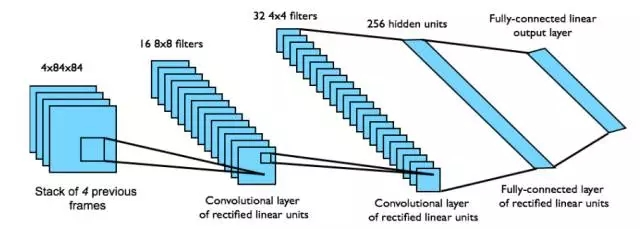
\includegraphics[width=4in]{dqn-atari.jpg}
\end{center}


\end{CJK*}
\end{document}